\documentclass[12pt]{article}
 
\usepackage[margin=1in]{geometry} 
\usepackage{amsmath,amsthm,amssymb}
\usepackage{hyperref}
\usepackage{graphicx}
\usepackage{xcolor}
\usepackage[many]{tcolorbox}
\tcbuselibrary{listings}
\usepackage{listings}
%jari:
\usepackage{enumitem}

\definecolor{lg}{HTML}{f0f0f0}

\newtcblisting{pycode}{
    colback=lg,
    boxrule=0pt,
    arc=0pt,
    outer arc=0pt,
    top=0pt,
    bottom=0pt,
    colframe=white,
    listing only,
    left=15.5pt,
    enhanced,
    listing options={
        basicstyle=\small\ttfamily,
        keywordstyle=\color{blue},
        language=Python,
        showstringspaces=false,
        tabsize=2,
        numbers=left,
        breaklines=true
    },
    overlay={
        \fill[gray!30]
        ([xshift=-3pt]frame.south west)
        rectangle
        ([xshift=11.5pt]frame.north west);
    }
}

\lstset{
    language=Python,
    basicstyle=\small\ttfamily,
}

 
\begin{document}
 
\title{Exercise 4}
\author{Jari Mattila - 35260T\\
ELEC-E8125 - Reinforcement Learning}

\maketitle

\section*{Task 1}

The training performance plots for Task 1a and 1b are presented below using 
handcrafted feature vector $\phi(s) = [s,|s|]^T$ in Figure~\ref*{fig:fig1} and 
using radial basis function representations in Figure~\ref*{fig:fig2}.
\newline

\begin{figure}[h] 
	\centering  % Remember to centre the figure
    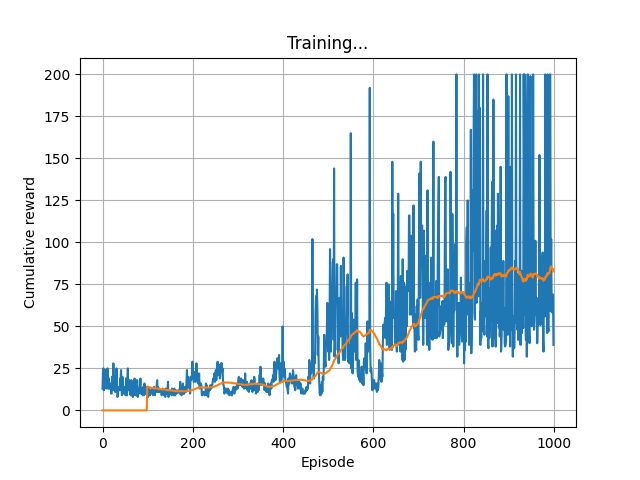
\includegraphics[width=0.9\columnwidth]{img/Figure_1_task_1a_cumulative_reward.png}
	\caption{Training performance using handcrafted feature vector $\phi(s) = [s,|s|]^T$.}
	\label{fig:fig1}
\end{figure}

\begin{figure}[h] 
	\centering  % Remember to centre the figure
    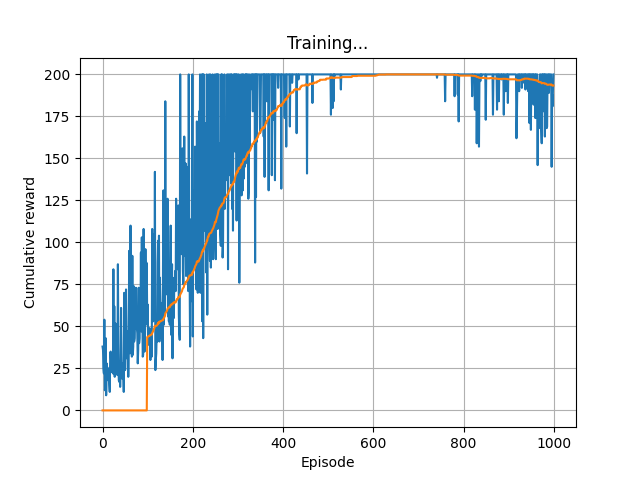
\includegraphics[width=0.9\columnwidth]{img/Figure_2_task_1b_cumulative_reward.png}
	\caption{Training performance using the GLIE formula for $\epsilon$.}
	\label{fig:fig2}
\end{figure}

\pagebreak


%\begin{itemize}
\begin{enumerate}[label=(\alph*)]
    \item handcrafted feature vector $\phi(s) = [s,|s|]^T$

Training plots of all methods (Task 1 a), b), Task 2 and Task 4).    
    
    \item radial basis function representations (use the featurizer inside the Agent class).

Training plots of all methods (Task 1 a), b), Task 2 and Task 4).
    
\end{enumerate}
%\end{itemize}


\noindent
Source files: qlearning.py, xx.py 

\section*{Question 1}

Would it be possible to learn accurately Q-values for the Cartpole
problem using linear features (by passing the state directly to a linear regressor)? Why/why
not?

\section*{Task 2}

Modify your Task 1 implementation to perform minibatch updates and
use experience replay (\textbf{while keeping the original code for Task 1 submission}) [1, p. 440].
Run the experiments with Cartpole with both feature representations.
\newline

Training plots of all methods (Task 1 a), b), Task 2 and Task 4).
\newline

\noindent
Source files: qlearning.py, xx.py 

\section*{Question 2}

Figure 2 shows the training performance of all four methods from Task 1, together
with grid-based learning from Exercise 3 evaluated using GLIE with a = 50.

\section*{Question 2.1}

How does the experience replay affect the learning performance?

\section*{Question 2.2}

Discuss the benefits and cons of using hand-crafted features. As an example, you can refer to 
the given hand-crafted feature and more complex features like
$\phi(s) = [s_x, s_{\dot{x}}, \operatorname{cos}(s_{\theta}), \operatorname{sin}(s_{\theta}), s_{\dot{\theta}}]^T$

\section*{Question 2.3}

Do grid based methods look sample-efficient compared to any of the
function approximation methods? Why/why not?

\section*{Task 3}

Create a 2D plot of policy (best action in terms of state) learned with RBF
with experience replay in terms of $x$ and $\theta$ for $\dot{x}=0$ and $\dot{\theta}=0$.
\newline

Policy plot from Task 3.
\newline

\noindent
Source files: qlearning.py, xx.py 

\section*{Task 4}

Replace the RBFs in your Task 2 implementation with a neural network
(\textbf{while keeping the original code for Task 2 submission}). A basic DQN implementation
can be found in dqn\_agent.py. Evaluate the method’s performance in CartPole and LunarLander
environments.
\newline

Training plots of all methods (Task 1 a), b), Task 2 and Task 4).
\newline

\noindent
Source files: qlearning.py, xx.py 

\section*{Question 3.1}

Can Q-learning be used directly in environments with continuous
action spaces?

\section*{Question 3.2}

Which steps of the algorithm would be difficult to compute in case of
a continuous action space? If any, what could be done to solve them?


\pagebreak

\section*{Final}

To embed code snippets in the report, you can use the \texttt{pycode} environment.

\begin{pycode}
for episode_number in range(train_episodes):
    reward_sum, timesteps = 0, 0
    done = False
    # Reset the environment and observe the initial state
    observation = env.reset()

    # Loop until the episode is over
    while not done:
        # Get action from the agent
        action, action_probabilities = agent.get_action(observation)
        previous_observation = observation

        # Perform the action on the environment, get new state and reward
        observation, reward, done, info = env.step(action)

        # Store action's outcome (so that the agent can improve its policy)
        agent.store_outcome(previous_observation, action_probabilities, action, reward)

        # Draw the frame, if desired
        if render:
            env.render()
\end{pycode}

If you add a figure, you can refer to it using Figure.~\ref*{fig:fig1}.

\begin{figure}[h] 
	\centering  % Remember to centre the figure
    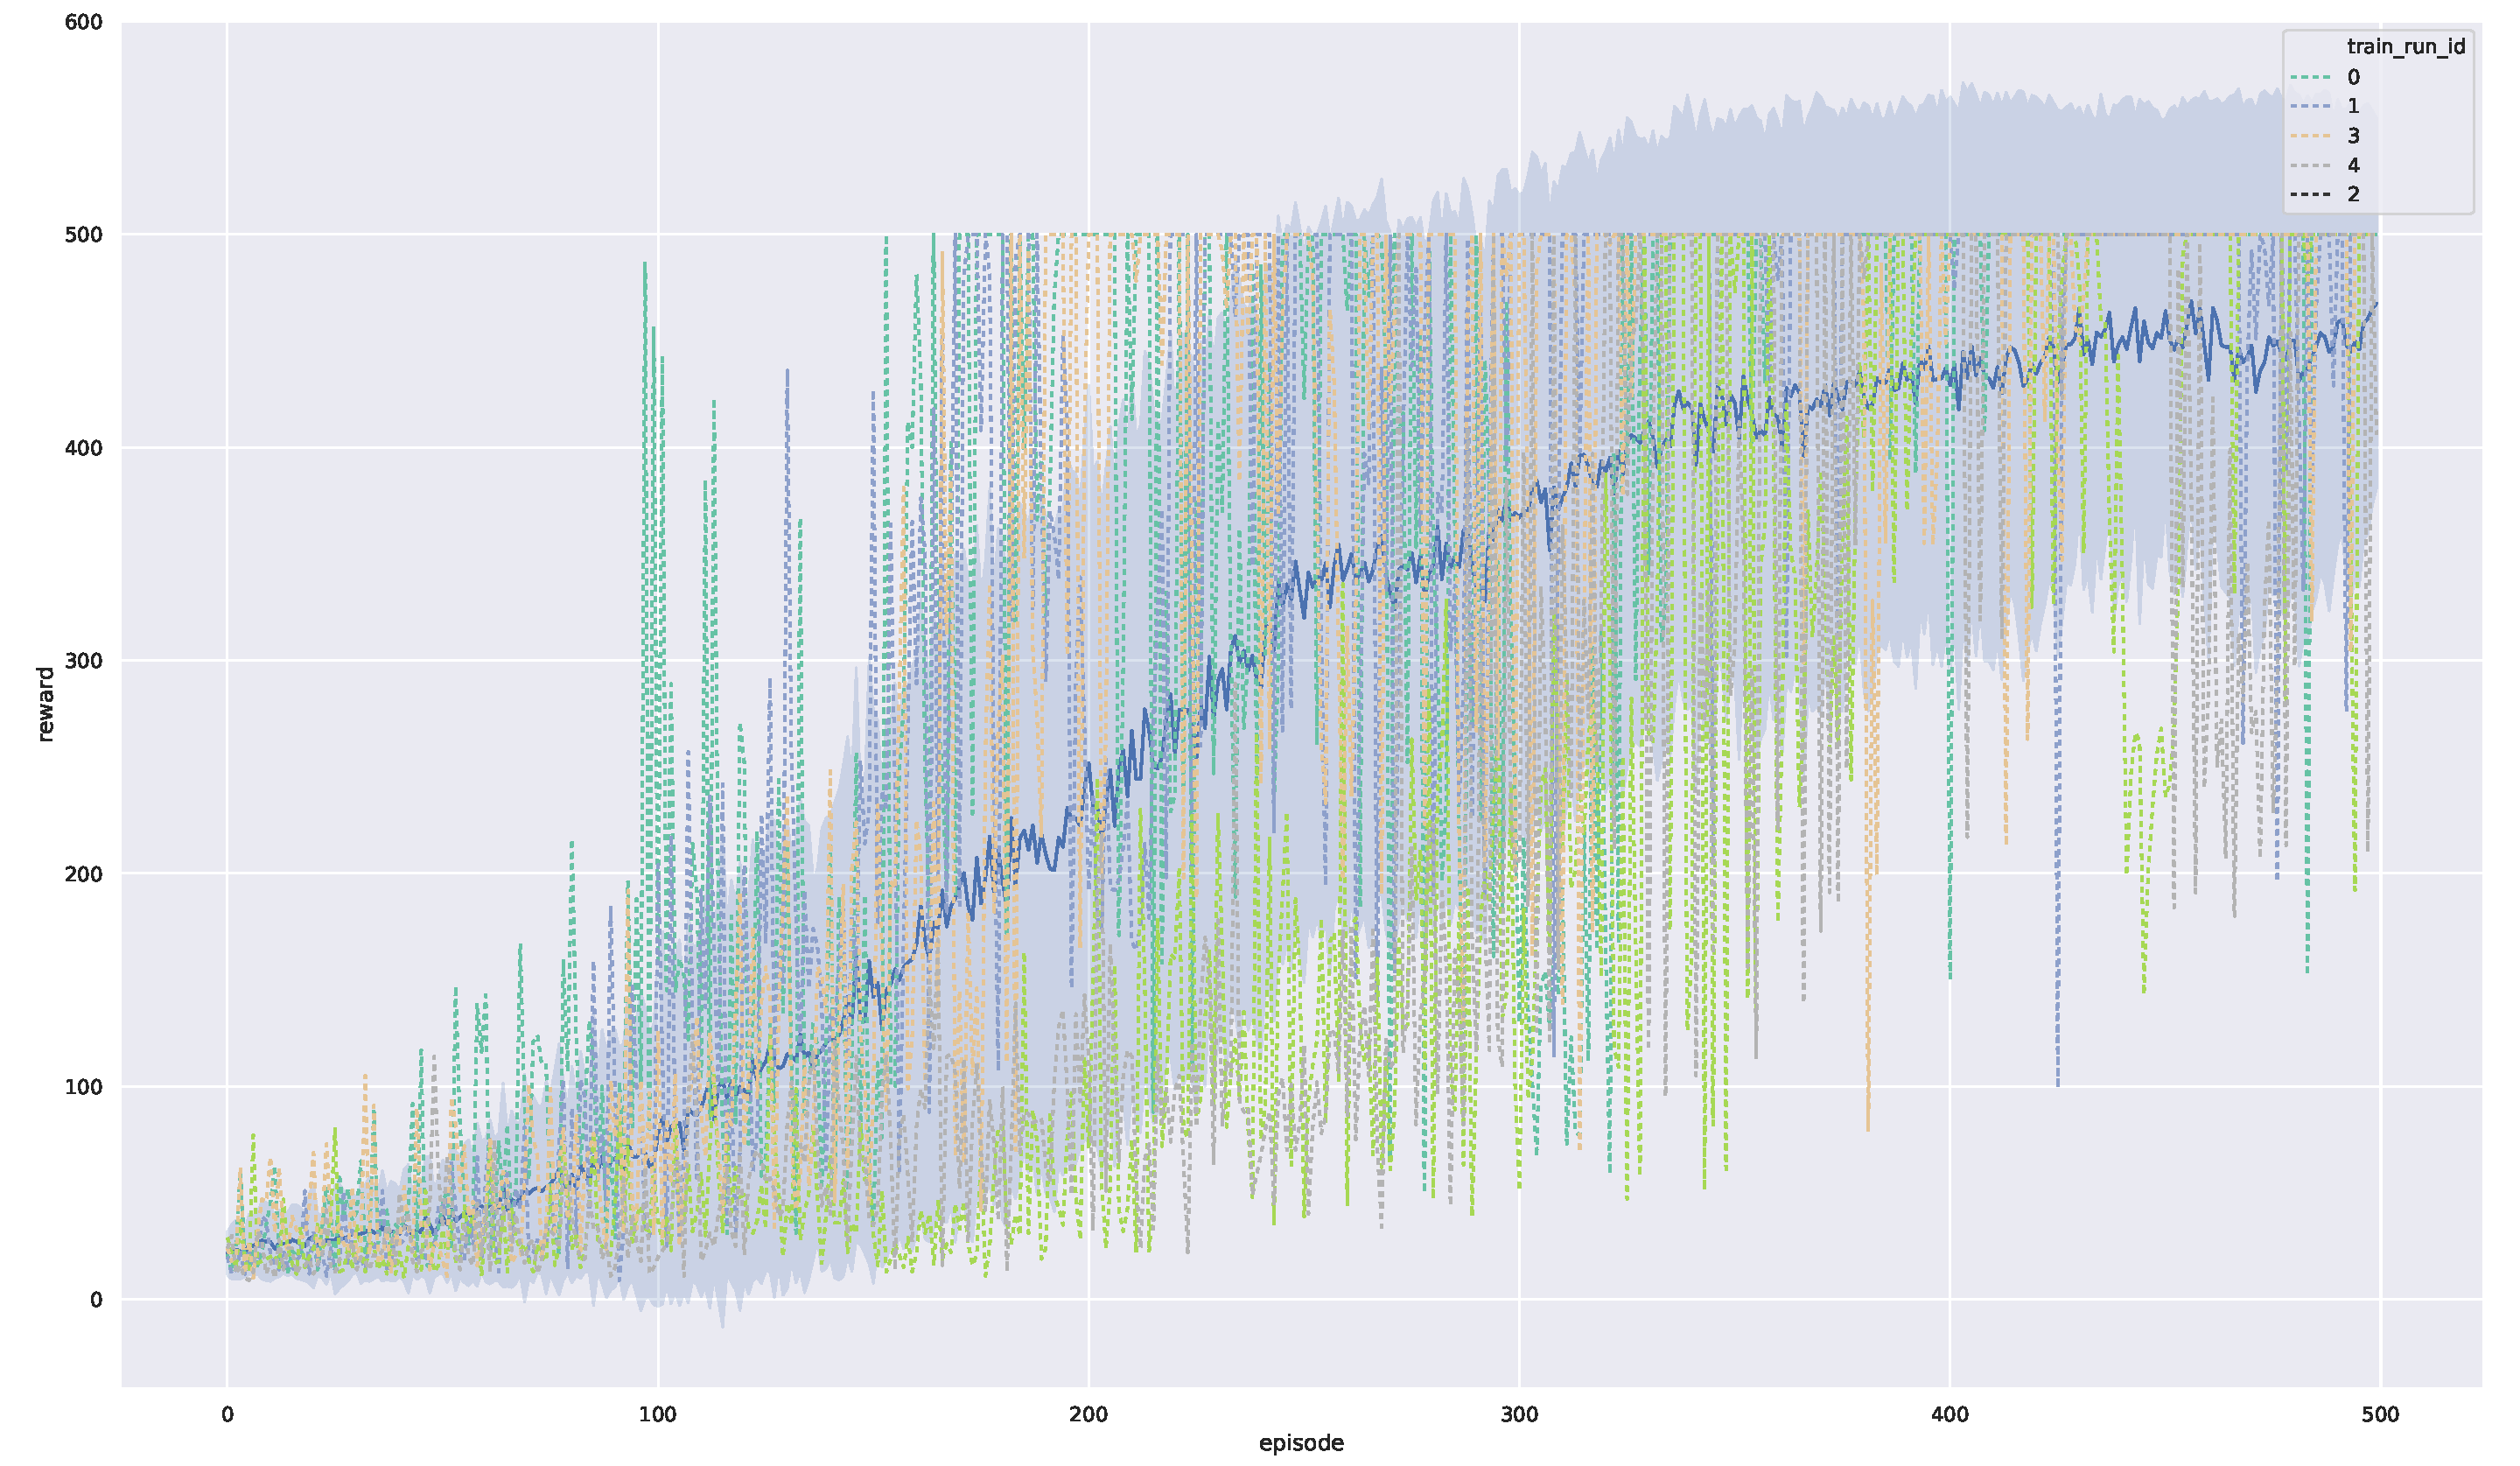
\includegraphics[width=0.9\columnwidth]{img/training.pdf}
	\caption{This is a sample figure.}
	\label{fig:fig1}
\end{figure}

\bibliographystyle{ieeetr}
\bibliography{template}  % Modify template with your bibliography name
\end{document}
